% =============================================================================
% Module 1e: Linearized Gravity and the Weak-Field Metric
% =============================================================================
% Sources: Carroll Ch. 4.1 (Newtonian limit), Ch. 7.1 (linearized gravity);
%          Congdon & Keeton Ch. 3.4 (weak-field light propagation)
% Mathematica: ../Mathematica/01e_Linearized_Gravity/
% =============================================================================

\chapter{Linearized Gravity and the Weak-Field Metric}
\label{ch:linearized_gravity}

\begin{quote}
\textit{In the weak-field limit, we can expand the metric about flat
spacetime and treat gravity as a small perturbation.  This is the regime
in which essentially all gravitational lensing takes place.}
\hfill --- Sean Carroll, \textit{Spacetime and Geometry}
\end{quote}

\noindent
In Modules~1a--1d we developed the full machinery of general relativity
and applied it to the exact Schwarzschild solution.  That framework is
necessary for understanding black holes and strong-field orbits, but
\textit{most gravitational lensing} --- by galaxies, galaxy clusters,
and large-scale structure --- operates in a regime where gravity is
weak: the Newtonian potential satisfies $|\Phi|/c^2 \ll 1$ and peculiar
velocities are small compared to $c$.  In this regime the metric can be
treated as a small perturbation of flat Minkowski spacetime, and the
resulting \textbf{linearized gravity} formalism is both simpler and
more directly connected to the lens equation that we will develop in
Module~4.

This module derives the weak-field metric from first principles, recovers
Newtonian gravity as a limiting case, computes the deflection of light
(reproducing the famous factor-of-two over the Newtonian prediction),
and introduces the effective refractive index interpretation that
provides the physical intuition behind Fermat's principle for lensing.
The linearity of the perturbation equations also guarantees that
deflection angles from multiple masses \textit{superpose} --- the
foundation for treating extended mass distributions in later modules.

\medskip
\noindent
\textbf{Companion Mathematica files:}
\begin{itemize}[nosep]
    \item \mathlink{01e_Linearized_Gravity/weak_field_metric.wl}{weak\_field\_metric.wl}
          --- symbolic verification of the Newtonian limit, weak-field
          deflection angle, factor-of-2, and figure generation
    \item \mathlink{01e_Linearized_Gravity/deflection_comparison.nb}{deflection\_comparison.nb}
          --- interactive comparison of exact Schwarzschild deflection
          vs.\ weak-field approximation; effective refractive index
          visualization
\end{itemize}


% =====================================================================
\section{Introduction: Why Linearize?}
\label{sec:why_linearize}

Consider a photon passing the Sun at the solar limb.  The relevant
dimensionless quantity characterizing the strength of gravity is
(Carroll eq.~4.11):
\begin{equation}
    \frac{|\Phi|}{c^2} = \frac{GM}{rc^2} \bigg|_{r = R_\odot}
    \approx \frac{6.674 \times 10^{-11} \times 1.989 \times 10^{30}}
    {6.96 \times 10^{8} \times (3 \times 10^{8})^2}
    \approx 2.1 \times 10^{-6} \,.
    \label{eq:sun_potential}
\end{equation}
For a typical galaxy lens ($M \sim 10^{12}\,\Msun$, $r \sim 10$~kpc),
the ratio is $|\Phi|/c^2 \sim 10^{-5}$ to $10^{-4}$.  Even for
galaxy clusters ($M \sim 10^{15}\,\Msun$, $r \sim 1$~Mpc), one finds
$|\Phi|/c^2 \sim 10^{-5}$.

In all of these astrophysical settings, gravity is \textit{extremely}
weak.  This justifies expanding the metric perturbatively around flat
spacetime and keeping only first-order terms --- the \textbf{linearized
gravity} approximation.

\begin{remark}
The only astrophysical setting where linearized gravity is
\textit{insufficient} for lensing is near black holes and neutron stars,
where $|\Phi|/c^2$ approaches unity.  Strong lensing by black holes
(e.g., the photon ring observed by the Event Horizon Telescope) requires
the full Schwarzschild or Kerr solution developed in Modules~1c and~1d.
\end{remark}


% =====================================================================
\section{The Weak-Field Expansion}
\label{sec:weak_field_expansion}

We write the full spacetime metric as a perturbation of the Minkowski
metric (Carroll eq.~7.1; Congdon \& Keeton eq.~3.68):
\begin{equation}
    \boxed{
    g_{\mu\nu} = \eta_{\mu\nu} + h_{\mu\nu} \,,
    \qquad |h_{\mu\nu}| \ll 1
    }
    \label{eq:metric_perturbation}
\end{equation}
where $\eta_{\mu\nu} = \mathrm{diag}(-1, +1, +1, +1)$ is the flat
Minkowski metric and $h_{\mu\nu}$ is the \textbf{metric perturbation}.
The condition $|h_{\mu\nu}| \ll 1$ means that spacetime is ``almost
flat'' --- deviations from Minkowski geometry are small.

The inverse metric to first order in $h$ is (Carroll eq.~7.2):
\begin{equation}
    g^{\mu\nu} = \eta^{\mu\nu} - h^{\mu\nu} + \order{h^2} \,,
    \label{eq:inverse_metric}
\end{equation}
where indices on $h_{\mu\nu}$ are raised and lowered with $\eta$.

The Christoffel symbols to first order are (Carroll eq.~7.4):
\begin{equation}
    \christoffel{\alpha}{\mu}{\nu}
    = \half \eta^{\alpha\beta}\bigl(
    \partial_\mu h_{\nu\beta} + \partial_\nu h_{\mu\beta}
    - \partial_\beta h_{\mu\nu}\bigr) + \order{h^2} \,.
    \label{eq:christoffel_linearized}
\end{equation}

\begin{remark}
In linearized gravity we systematically discard all terms of order
$h^2$ and higher.  This means the Christoffel symbols are first order
in $h$, the Riemann tensor is first order, and the Einstein equations
become \textit{linear} in $h_{\mu\nu}$.  Linearity is the crucial
simplification that allows superposition of gravitational effects.
\end{remark}


% =====================================================================
\section{The Newtonian Limit}
\label{sec:newtonian_limit}

We now show that the geodesic equation in the weak-field, slow-motion
limit reduces to Newton's second law, thereby identifying the metric
perturbation $h_{00}$ with the Newtonian potential $\Phi$.

\subsection{Assumptions}

The \textbf{Newtonian limit} requires three conditions
(Carroll Sec.~4.1):
\begin{enumerate}
    \item \textbf{Weak field:} $|h_{\mu\nu}| \ll 1$
    \item \textbf{Slow motion:} $v \ll c$, so
          $dx^i/d\tau \ll dx^0/d\tau = c\,dt/d\tau$
    \item \textbf{Static field:} $\partial_0 h_{\mu\nu} = 0$
          (the gravitational field is not changing with time)
\end{enumerate}

\subsection{Derivation}

The geodesic equation for a massive particle is (Carroll eq.~3.44):
\begin{equation}
    \frac{d^2 x^\mu}{d\tau^2}
    + \christoffel{\mu}{\alpha}{\beta}\,
    \frac{dx^\alpha}{d\tau}\, \frac{dx^\beta}{d\tau} = 0 \,.
    \label{eq:geodesic_full}
\end{equation}
In the slow-motion limit, $dx^i/d\tau$ is negligible compared to
$dx^0/d\tau = c\,dt/d\tau$, so the double sum over $\alpha, \beta$
is dominated by the $\alpha = \beta = 0$ term:
\begin{equation}
    \frac{d^2 x^\mu}{d\tau^2}
    + \christoffel{\mu}{0}{0}\left(\frac{dx^0}{d\tau}\right)^{\!2}
    \approx 0 \,.
    \label{eq:geodesic_slow}
\end{equation}

From eq.~\eqref{eq:christoffel_linearized}, using the static-field
condition ($\partial_0 h_{\mu\nu} = 0$):
\begin{equation}
    \christoffel{\mu}{0}{0}
    = \half \eta^{\mu\alpha}\bigl(
    \partial_0 h_{0\alpha} + \partial_0 h_{0\alpha}
    - \partial_\alpha h_{00}\bigr)
    = -\half \eta^{\mu\alpha}\, \partial_\alpha h_{00} \,.
    \label{eq:gamma_00}
\end{equation}
For the spatial components ($\mu = i$), this gives
$\christoffel{i}{0}{0} = -\half \partial_i h_{00}$.

The spatial part of the geodesic equation then becomes:
\begin{equation}
    \frac{d^2 x^i}{d\tau^2}
    = \half \partial_i h_{00}\left(\frac{dx^0}{d\tau}\right)^{\!2}
    = \half c^2 \partial_i h_{00}\left(\frac{dt}{d\tau}\right)^{\!2} .
    \label{eq:geodesic_spatial}
\end{equation}
Using $d\tau \approx dt$ (valid for slow motion, since $\gamma \approx 1$),
we get:
\begin{equation}
    \frac{d^2 x^i}{dt^2} = \half c^2\, \partial_i h_{00} \,.
    \label{eq:newton_from_geodesic}
\end{equation}

\subsection{Identification with Newtonian Gravity}

Newton's second law in a gravitational field is:
\begin{equation}
    \frac{d^2 x^i}{dt^2} = -\partial_i \Phi \,.
    \label{eq:newton_law}
\end{equation}
Comparing with eq.~\eqref{eq:newton_from_geodesic}, we identify
(Carroll eq.~4.12):
\begin{equation}
    \boxed{
    h_{00} = -\frac{2\Phi}{c^2}
    }
    \label{eq:h00_identification}
\end{equation}
The time-time component of the metric perturbation is determined by the
Newtonian potential.  For a point mass $M$, $\Phi = -GM/r$, so:
\begin{equation}
    h_{00} = \frac{2GM}{c^2 r} = \frac{R_S}{r} \,,
    \label{eq:h00_point_mass}
\end{equation}
where $R_S = 2GM/c^2$ is the Schwarzschild radius.

\begin{exercise}
\label{ex:newtonian_limit}
Starting from the geodesic equation~\eqref{eq:geodesic_full} with the
perturbed metric $g_{\mu\nu} = \eta_{\mu\nu} + h_{\mu\nu}$, carry out
the Newtonian limit derivation in full detail.  Show that for
slow-moving particles in a static, weak gravitational field:
\begin{enumerate}[label=(\alph*)]
    \item The only relevant Christoffel symbol is
          $\christoffel{i}{0}{0} = -\half \partial_i h_{00}$.
    \item The geodesic equation reduces to
          $d^2 x^i / dt^2 = \half c^2\, \partial_i h_{00}$.
    \item Comparing with Newton's law identifies
          $h_{00} = -2\Phi/c^2$.
\end{enumerate}
Verify each step using
\mathlink{01e_Linearized_Gravity/weak_field_metric.wl}{weak\_field\_metric.wl}.
\end{exercise}


% =====================================================================
\section{The Weak-Field Metric}
\label{sec:weak_field_metric}

The Newtonian limit only determined $h_{00}$.  To get the full
weak-field metric --- including the spatial components needed for
light bending --- we must go beyond the slow-motion assumption and
use the linearized Einstein equations.

For a static, spherically symmetric source, the solution to the
linearized Einstein equations in isotropic coordinates gives
(Congdon \& Keeton eq.~3.71; Carroll eq.~7.8):
\begin{equation}
    \boxed{
    ds^2 = -\left(1 + \frac{2\Phi}{c^2}\right) c^2\, dt^2
    + \left(1 - \frac{2\Phi}{c^2}\right)
    \bigl(dx^2 + dy^2 + dz^2\bigr)
    }
    \label{eq:weak_field_metric}
\end{equation}
where $\Phi(\mathbf{x})$ is the Newtonian gravitational potential
(with $\Phi < 0$ for attractive gravity).  Equivalently:
\begin{equation}
    h_{00} = -\frac{2\Phi}{c^2} \,, \qquad
    h_{ij} = -\frac{2\Phi}{c^2}\,\delta_{ij} \,.
    \label{eq:h_components}
\end{equation}

\begin{remark}
The key point is that \textbf{both} the time and space components of
the metric are perturbed, and by equal amounts.  The Newtonian limit
(which assumes slow motion) only probes $h_{00}$, because the spatial
components of the four-velocity are negligible.  But photons travel at
$c$, so all components of the metric contribute equally to the
propagation of light.  This is why light bending in GR is
\textit{twice} the Newtonian prediction.
\end{remark}

\begin{exercise}
\label{ex:schwarzschild_weak_field}
The Schwarzschild metric in standard coordinates is:
\[
    ds^2 = -\left(1 - \frac{R_S}{r}\right) c^2 dt^2
    + \left(1 - \frac{R_S}{r}\right)^{-1} dr^2
    + r^2\, d\Omega^2 \,.
\]
\begin{enumerate}[label=(\alph*)]
    \item Expand $(1 - R_S/r)^{-1} \approx 1 + R_S/r + \order{(R_S/r)^2}$
          and show that the metric becomes:
          \[
              ds^2 \approx -\left(1 - \frac{R_S}{r}\right) c^2 dt^2
              + \left(1 + \frac{R_S}{r}\right) dr^2
              + r^2\, d\Omega^2 \,.
          \]
    \item Transform to Cartesian-like coordinates and show that this
          matches the weak-field metric~\eqref{eq:weak_field_metric}
          with $\Phi = -GM/r$ to first order in $R_S/r$.
\end{enumerate}
Verify with
\mathlink{01e_Linearized_Gravity/weak_field_metric.wl}{weak\_field\_metric.wl}.
\end{exercise}


% =====================================================================
\section{Null Geodesics in the Weak-Field Metric}
\label{sec:null_geodesics_weak}

We now derive the deflection of light in the weak-field metric.  This
is the central result of this module and the starting point for the
entire gravitational lensing formalism.

\subsection{Setup}

Consider a photon propagating through the weak-field
metric~\eqref{eq:weak_field_metric} generated by a point mass $M$ at
the origin, with $\Phi = -GM/r$.  The photon travels along a null
geodesic: $ds^2 = 0$.

For a photon moving primarily in the $x$-direction, passing the mass
at impact parameter $b$ (the closest approach distance in the absence
of deflection), we can use the \textbf{Born approximation}: compute
the deflection along the unperturbed (straight-line) path.  This is
valid when the deflection angle is small, which is guaranteed by the
weak-field condition.

\subsection{The Null Condition}

Setting $ds^2 = 0$ in eq.~\eqref{eq:weak_field_metric}:
\begin{equation}
    \left(1 + \frac{2\Phi}{c^2}\right) c^2 dt^2
    = \left(1 - \frac{2\Phi}{c^2}\right)
    \bigl(dx^2 + dy^2 + dz^2\bigr) \,.
    \label{eq:null_condition}
\end{equation}
The coordinate speed of light is therefore:
\begin{equation}
    \frac{|\mathbf{dx}|}{dt}
    = c\,\sqrt{\frac{1 + 2\Phi/c^2}{1 - 2\Phi/c^2}}
    \approx c\left(1 + \frac{2\Phi}{c^2}\right)
    \label{eq:coordinate_speed}
\end{equation}
to first order in $\Phi/c^2$.  Since $\Phi < 0$, the coordinate speed
is \textit{less} than $c$ near a mass --- gravity slows light.

\subsection{Deflection Angle}

The deflection due to the temporal perturbation $h_{00}$ alone is
computed by integrating the transverse gradient of $|\Phi|$ along the
unperturbed (straight-line) path (Congdon \& Keeton eq.~3.77):
\begin{equation}
    \alphahat_{\mathrm{time}} = \frac{2}{c^2} \int_{-\infty}^{+\infty}
    \nabla_\perp |\Phi|\, dl \,,
    \label{eq:deflection_integral_half}
\end{equation}
where $\nabla_\perp$ denotes the gradient of $|\Phi|$ perpendicular to
the photon's path and $dl$ is the path length along the unperturbed
trajectory.  This gives the ``Newtonian'' contribution to the
deflection.

The spatial perturbation $h_{ij}$ contributes an \textit{equal} amount,
doubling the result.  In the PPN (parametrized post-Newtonian)
formalism, the full deflection angle is written as
(Congdon \& Keeton eq.~3.78; Will 1993):
\begin{equation}
    \boxed{
    \alphahat = \frac{1 + \gamma_{\mathrm{PPN}}}{c^2}
    \int_{-\infty}^{+\infty} \nabla_\perp |\Phi|\, dl
    }
    \label{eq:deflection_integral}
\end{equation}
where $\gamma_{\mathrm{PPN}} = 1$ in GR (the PPN parameter measuring
the spatial curvature contribution).  The Newtonian prediction
corresponds to $\gamma_{\mathrm{PPN}} = 0$, giving half the GR value.

\subsection{Point Mass Deflection}

For a point mass with $|\Phi| = GM/r$, the photon travels along the
$x$-axis at perpendicular distance $b$ (so
$r = \sqrt{x^2 + b^2}$ and
$\nabla_\perp |\Phi| = (GM\, b)/(x^2 + b^2)^{3/2}$).
The line-of-sight integral evaluates to:
\begin{equation}
    \int_{-\infty}^{+\infty} \nabla_\perp |\Phi|\, dl
    = GM \int_{-\infty}^{+\infty}
    \frac{b\, dx}{(x^2 + b^2)^{3/2}}
    = GM \cdot \frac{2}{b}
    = \frac{2GM}{b} \,,
    \label{eq:deflection_integral_eval}
\end{equation}
using the standard integral
$\int_{-\infty}^{+\infty} b\, dx/(x^2 + b^2)^{3/2} = 2/b$.
With $\gamma_{\mathrm{PPN}} = 1$ (GR), the deflection angle is:
\begin{equation}
    \boxed{
    \alphahat = \frac{4GM}{c^2 b}
    }
    \label{eq:deflection_point_mass}
\end{equation}
This is the \textbf{Einstein deflection angle} for a point mass ---
the single most important equation in gravitational lensing.  We derived
this here via the Born approximation in the weak-field metric; in
Module~\ref{ch:light_deflection} we will re-derive it from the exact null
geodesic orbit equation in the full Schwarzschild metric, confirming
that both approaches agree.

\begin{figure}[ht]
    \centering
    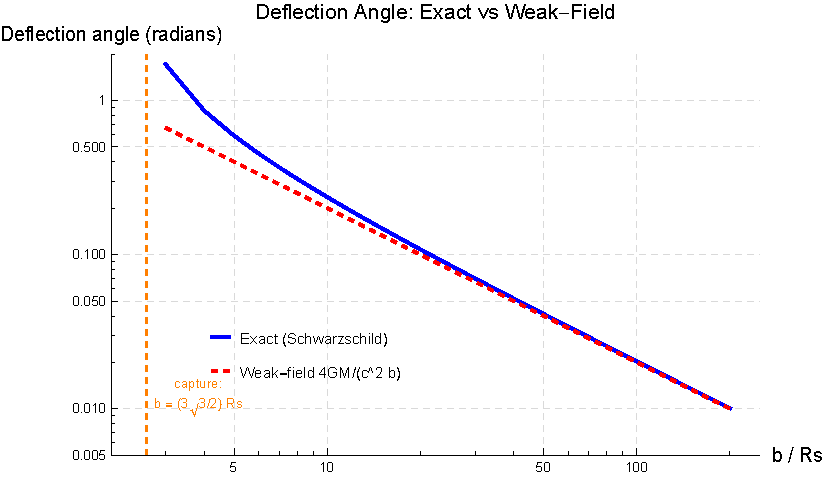
\includegraphics[width=0.70\textwidth]{../Figures/01e_Linearized_Gravity/deflection_comparison.pdf}
    \caption{Comparison of the exact Schwarzschild deflection angle
    (solid blue) with the weak-field approximation
    $\alphahat = 4GM/(c^2 b)$ (dashed red) as a function of impact
    parameter $b/R_S$.  The two curves are virtually indistinguishable
    for $b/R_S \gtrsim 5$ (i.e., $|\Phi|/c^2 \lesssim 0.1$).  For the
    Sun, $R_S \approx 3$~km and the closest approach is $R_\odot \approx
    7 \times 10^5$~km, so $b/R_S \sim 2 \times 10^5$ --- deep in the
    weak-field regime.  Interactive version:
    \texttt{deflection\_comparison.nb}.
    (cf.\ Congdon \& Keeton Fig.~3.7)}
    \label{fig:deflection_comparison}
\end{figure}

\subsection{The Factor of Two}

The factor of 4 in eq.~\eqref{eq:deflection_point_mass} (rather than 2)
is one of the most celebrated results in GR.  Its origin is as follows:
\begin{itemize}
    \item The temporal perturbation $h_{00} = -2\Phi/c^2$ contributes a
          deflection of $2GM/(c^2 b)$.  This is the ``Newtonian'' part,
          which can also be derived by treating the photon as a
          Newtonian particle moving at speed $c$.
    \item The spatial perturbation $h_{ij} = -2\Phi/c^2\, \delta_{ij}$
          contributes an \textit{equal} additional deflection of
          $2GM/(c^2 b)$.  This arises because photons, unlike massive
          particles, are equally sensitive to the spatial curvature.
\end{itemize}
The total is $4GM/(c^2 b) = 2 \times (2GM/(c^2 b))$, i.e., \textbf{twice
the Newtonian prediction}.  This factor of 2 was confirmed by
Eddington's 1919 solar eclipse expedition and is one of the classical
tests of general relativity.

\begin{remark}
Historically, Einstein himself initially published the ``Newtonian''
value $2GM/(c^2 b)$ in 1911, before he had completed general
relativity.  The correct value $4GM/(c^2 b)$ appeared in 1915, after
Einstein accounted for the spatial curvature.  The Eddington expedition
confirmed the GR value, not the 1911 prediction.
\end{remark}

\begin{exercise}
\label{ex:deflection_derivation}
Derive the Einstein deflection angle $\alphahat = 4GM/(c^2 b)$ for a
point mass by evaluating the integral~\eqref{eq:deflection_integral}
with $|\Phi| = GM/r$ along the unperturbed photon path
$\mathbf{x}(l) = (l, b, 0)$.
\begin{enumerate}[label=(\alph*)]
    \item Show that $\nabla_\perp |\Phi| = (GM\, b)/(l^2 + b^2)^{3/2}$.
    \item Evaluate
          $\int_{-\infty}^{\infty} b\, dl/(l^2 + b^2)^{3/2} = 2/b$.
    \item Combine with $\gamma_{\mathrm{PPN}} = 1$ to obtain
          $\alphahat = 4GM/(c^2 b)$.
    \item Compute $\alphahat$ for the Sun at the solar limb
          ($b = R_\odot = 6.96 \times 10^8$~m) and verify
          $\alphahat \approx 1.75''$.
\end{enumerate}
Check with
\mathlink{01e_Linearized_Gravity/weak_field_metric.wl}{weak\_field\_metric.wl}.
\end{exercise}


% =====================================================================
\section{The Effective Refractive Index}
\label{sec:refractive_index}

The weak-field metric leads to a beautiful analogy between gravitational
lensing and optics.  From eq.~\eqref{eq:coordinate_speed}, the
coordinate speed of light near a mass is:
\begin{equation}
    v_{\mathrm{coord}} = c\left(1 + \frac{2\Phi}{c^2}\right) \,.
    \label{eq:coord_speed_light}
\end{equation}
We can define an \textbf{effective refractive index} by analogy with
optics, where $v = c/n$:
\begin{equation}
    \boxed{
    n(\mathbf{x}) = \frac{c}{v_{\mathrm{coord}}}
    \approx 1 - \frac{2\Phi}{c^2}
    = 1 + \frac{2|\Phi|}{c^2}
    }
    \label{eq:refractive_index}
\end{equation}
Since $\Phi < 0$ near a mass, $n > 1$: gravity acts as a medium with
refractive index greater than unity, \textit{slowing} light (in
coordinate time) and bending it toward the mass.

\begin{figure}[ht]
    \centering
    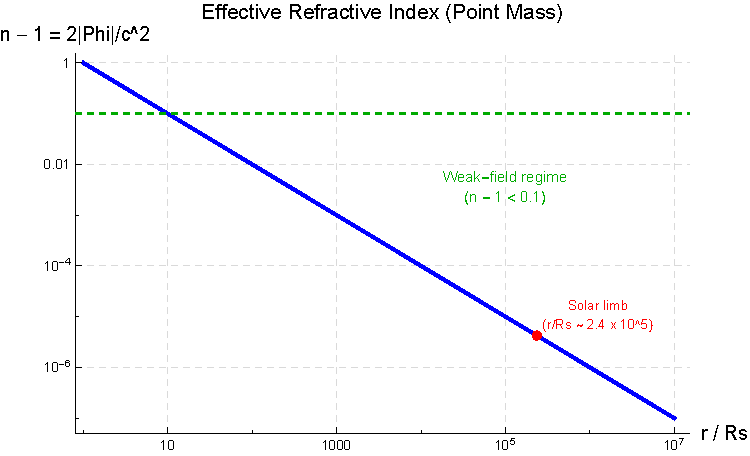
\includegraphics[width=0.65\textwidth]{../Figures/01e_Linearized_Gravity/refractive_index.pdf}
    \caption{Effective refractive index $n = 1 + 2|\Phi|/c^2$ as a
    function of distance from a point mass, plotted for a solar-mass
    object.  The refractive index is largest (light is slowest) at the
    surface of the mass and approaches unity far away.}
    \label{fig:refractive_index}
\end{figure}

This refractive index interpretation has two important consequences:

\paragraph{Fermat's Principle.}
In optics, light follows the path that extremizes the optical path
length $\int n\, dl$.  The same principle applies in gravitational
lensing: photons follow paths that extremize the
\textbf{time delay functional} (Carroll eq.~7.47;
Congdon \& Keeton eq.~6.1):
\begin{equation}
    t[\mathbf{x}(l)] = \frac{1}{c} \int n\, dl
    = \frac{1}{c} \int \left(1 + \frac{2|\Phi|}{c^2}\right) dl \,.
    \label{eq:fermat_principle}
\end{equation}
This will be the foundation for the time delay formalism in Module~6.

\paragraph{Shapiro Time Delay.}
Light passing near a mass arrives later than it would in flat spacetime,
by an amount proportional to $\int 2|\Phi|/c^2\, dl$ along the path.
This \textbf{Shapiro delay} has been measured to high precision using
radar signals bouncing off Mercury and Venus.

\begin{exercise}
\label{ex:refractive_index}
Compute the effective refractive index $n$ at the following distances
from the Sun ($M = \Msun$):
\begin{enumerate}[label=(\alph*)]
    \item The solar surface ($r = R_\odot = 6.96 \times 10^8$~m)
    \item The Earth's orbit ($r = 1$~AU $= 1.496 \times 10^{11}$~m)
    \item The orbit of Pluto ($r = 39.5$~AU)
\end{enumerate}
For each, compute $n - 1 = 2GM/(c^2 r)$ and comment on the magnitude.
\end{exercise}


% =====================================================================
\section{Superposition in Linearized Gravity}
\label{sec:superposition}

Because the metric perturbation $h_{\mu\nu}$ satisfies \textit{linear}
equations in the weak-field limit, we can superpose solutions.  If we
have two masses $M_1$ and $M_2$ at positions $\mathbf{x}_1$ and
$\mathbf{x}_2$, the total Newtonian potential is:
\begin{equation}
    \Phi(\mathbf{x}) = -\frac{GM_1}{|\mathbf{x} - \mathbf{x}_1|}
    - \frac{GM_2}{|\mathbf{x} - \mathbf{x}_2|} \,,
    \label{eq:superposition_potential}
\end{equation}
and the total deflection angle is simply the \textit{vector sum} of
the individual deflections:
\begin{equation}
    \boxed{
    \boldsymbol{\hat{\alpha}} = \sum_i \frac{4GM_i}{c^2}\,
    \frac{\vecxi - \vecxi_i}{|\vecxi - \vecxi_i|^2}
    }
    \label{eq:superposition_deflection}
\end{equation}
where $\vecxi$ is the position in the lens plane and $\vecxi_i$
is the projected position of mass $M_i$.

For a continuous mass distribution with surface mass density
$\Sigma(\vecxi)$, this becomes (Congdon \& Keeton eq.~4.5):
\begin{equation}
    \boldsymbol{\hat{\alpha}}(\vecxi) = \frac{4G}{c^2}
    \int \frac{(\vecxi - \vecxi')\, \Sigma(\vecxi')}
    {|\vecxi - \vecxi'|^2}\, d^2\xi' \,.
    \label{eq:continuous_deflection}
\end{equation}
This integral is the starting point for all lens models in Modules~7--10.

\begin{remark}
Superposition of deflection angles does \textit{not} hold in the
exact (nonlinear) theory.  It is a consequence of linearization and is
valid only when all masses satisfy $|\Phi|/c^2 \ll 1$.  Fortunately,
this condition is satisfied for essentially all astrophysical lensing
systems.
\end{remark}

\begin{exercise}
\label{ex:superposition}
Two point masses $M_1 = M_2 = M$ are located at
$\mathbf{x}_1 = (-d/2, 0)$ and $\mathbf{x}_2 = (+d/2, 0)$ in the
lens plane.  A photon passes through the midpoint at
$\vecxi = (0, b)$.
\begin{enumerate}[label=(\alph*)]
    \item Write down the deflection angle vector from each mass.
    \item Show that the $x$-components cancel by symmetry and that the
          total deflection is:
          \[
              \hat{\alpha}_y = \frac{8GMb}{c^2(d^2/4 + b^2)} \,.
          \]
    \item Verify that in the limit $d \to 0$ (masses merge) this
          reduces to $\hat{\alpha} = 8GM/(c^2 b) = 4G(2M)/(c^2 b)$,
          i.e., the deflection by a single mass of $2M$.
\end{enumerate}
Check with
\solnlink{01e_Linearized_Gravity/problems\_01e.wl}{problems\_01e.wl}.
\end{exercise}


% =====================================================================
\section{Preview: From Deflection to the Lens Equation}
\label{sec:preview_lens_equation}

The deflection angle~\eqref{eq:deflection_point_mass} is a
\textit{physical} angle, measured in the frame of the lens.  To connect
this to observed image positions on the sky, we need the
\textbf{lens equation}, which relates the true source position
$\vecbeta$ to the observed image position $\vectheta$ through the
deflection angle (Congdon \& Keeton eq.~4.1):
\begin{equation}
    \vecbeta = \vectheta - \frac{\Dds}{\Ds}\, \vecalpha(\vectheta) \,,
    \label{eq:lens_equation_preview}
\end{equation}
where $\vecalpha = (\Dd / \Ds)\, \boldsymbol{\hat{\alpha}}$ is the
\textbf{reduced deflection angle} and $\Dd$, $\Ds$, $\Dds$ are the
angular diameter distances from observer to lens, observer to source,
and lens to source.

The full derivation of this equation, along with the thin-lens
approximation and the definition of angular diameter distances, will be
developed in Modules~3 and~4.  The key point for now is that the
weak-field deflection angle computed in this module provides the
essential input to the lens equation.

\begin{figure}[ht]
    \centering
    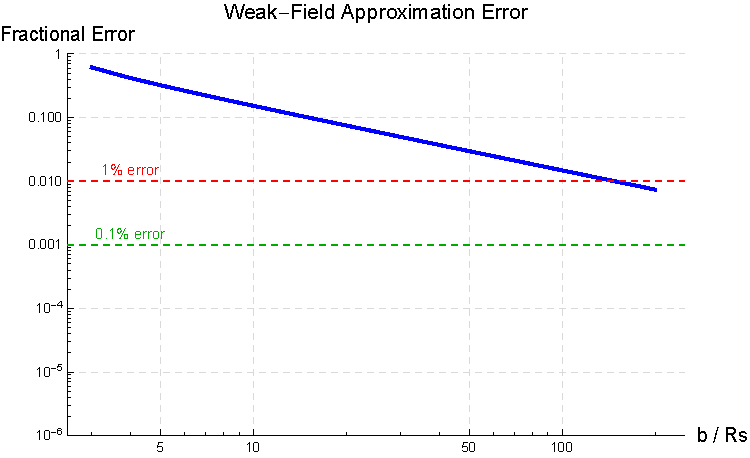
\includegraphics[width=0.75\textwidth]{../Figures/01e_Linearized_Gravity/exact_vs_weak_field.pdf}
    \caption{Fractional error $|\alphahat_{\mathrm{exact}} -
    \alphahat_{\mathrm{weak}}| / \alphahat_{\mathrm{exact}}$ of the
    weak-field approximation as a function of $b/R_S$.  The error is
    below 1\% for $b/R_S \gtrsim 50$ and below 0.1\% for
    $b/R_S \gtrsim 150$.  For typical astrophysical lenses
    ($b/R_S > 10^4$), the weak-field approximation is essentially
    exact.}
    \label{fig:exact_vs_weak_field}
\end{figure}


% =====================================================================
\section{Summary}
\label{sec:linearized_summary}

\begin{itemize}
    \item In the weak-field limit, the metric is
          $g_{\mu\nu} = \eta_{\mu\nu} + h_{\mu\nu}$ with
          $|h_{\mu\nu}| \ll 1$.

    \item The Newtonian limit of the geodesic equation identifies
          $h_{00} = -2\Phi/c^2$, where $\Phi$ is the Newtonian
          gravitational potential.

    \item The full weak-field metric has \textit{equal} perturbations in
          time and space:
          $ds^2 = -(1 + 2\Phi/c^2)\,c^2 dt^2 + (1 - 2\Phi/c^2)\,
          d\mathbf{x}^2$.

    \item Null geodesics in this metric yield the Einstein deflection
          angle $\alphahat = 4GM/(c^2 b)$ --- \textbf{twice} the
          Newtonian value.  The factor of 2 arises from the spatial
          curvature contribution.

    \item The weak-field metric defines an effective refractive index
          $n = 1 + 2|\Phi|/c^2 > 1$, connecting gravitational lensing
          to Fermat's principle and the Shapiro time delay.

    \item Linearized gravity allows \textbf{superposition}: deflection
          angles from multiple masses add vectorially.  This is the
          foundation for treating galaxies, clusters, and continuous
          mass distributions as gravitational lenses.

    \item The deflection angle is the key input to the lens equation
          (Module~4), which maps source positions to image positions.
\end{itemize}


% =====================================================================
\section{Problems}
\label{sec:linearized_problems}

\begin{exercise}
\label{ex:newtonian_limit_prob}
\textbf{(Newtonian limit from the geodesic equation.)}
Carry out the full Newtonian limit derivation described in
Section~\ref{sec:newtonian_limit}.  Starting from the geodesic
equation with $g_{\mu\nu} = \eta_{\mu\nu} + h_{\mu\nu}$:
\begin{enumerate}[label=(\alph*)]
    \item Compute the Christoffel symbol $\christoffel{i}{0}{0}$ to
          first order in $h$.
    \item Apply the slow-motion and static-field approximations.
    \item Show that $d^2 x^i/dt^2 = -\partial_i \Phi$ implies
          $h_{00} = -2\Phi/c^2$.
\end{enumerate}
\end{exercise}

\begin{exercise}
\label{ex:weak_field_schwarzschild}
\textbf{(Weak-field Schwarzschild.)}
Expand the Schwarzschild metric to first order in $R_S/r$ and verify
that it matches the weak-field metric~\eqref{eq:weak_field_metric}
with $\Phi = -GM/r$.  Specifically:
\begin{enumerate}[label=(\alph*)]
    \item Expand $(1 - R_S/r)^{-1} \approx 1 + R_S/r$.
    \item Write the result in isotropic Cartesian coordinates.
    \item Identify $h_{00} = R_S/r$ and $h_{ij} = (R_S/r)\,\delta_{ij}$
          and confirm $h_{00} = h_{ij}/\delta_{ij}$.
\end{enumerate}
\end{exercise}

\begin{exercise}
\label{ex:refractive_index_prob}
\textbf{(Effective refractive index.)}
Compute the effective refractive index $n = 1 + 2|\Phi|/c^2$ for a
point mass $M = \Msun$ at distances:
(a) $r = R_\odot$,
(b) $r = 1$~AU,
(c) $r = 1$~kpc.
Comment on whether the weak-field approximation is valid in each case.
\end{exercise}

\begin{exercise}
\label{ex:deflection_angle_derivation}
\textbf{(Deflection angle from null geodesics.)}
Derive $\alphahat = 4GM/(c^2 b)$ by evaluating the
integral~\eqref{eq:deflection_integral} with $\gamma_{\mathrm{PPN}} = 1$
for a point mass along the unperturbed path.  Compute the deflection angle for:
(a) the Sun at the solar limb,
(b) a $10^{12}\,\Msun$ galaxy at $b = 10$~kpc.
Express results in arcseconds.
\end{exercise}

\begin{exercise}
\label{ex:superposition_prob}
\textbf{(Superposition of deflection angles.)}
Two equal point masses $M$ are separated by distance $d$ in the lens
plane.
\begin{enumerate}[label=(\alph*)]
    \item Derive the total deflection angle for a photon passing at
          perpendicular distance $b$ from the midpoint (along the
          symmetry axis perpendicular to the line joining the masses).
    \item Show that for $b \gg d$, the result approaches
          $\alphahat \to 4G(2M)/(c^2 b)$: at large distances the two
          masses act as a single mass $2M$.
    \item Plot $\hat{\alpha}(b)$ for $d = 1$~kpc and
          $M = 10^{11}\,\Msun$ using Mathematica.
\end{enumerate}
\end{exercise}
